% !TEX program = pdflatex
\documentclass[aspectratio=169,11pt]{beamer}

% ── Theme ──
\usetheme{metropolis}
\usecolortheme{default}
\setbeamertemplate{navigation symbols}{}
\setbeamertemplate{footline}[frame number]

% ── Packages ──
\usepackage{booktabs}
\usepackage{graphicx}
\usepackage{amsmath,amssymb}
\usepackage{tikz}
\usetikzlibrary{arrows.meta,positioning,shapes,calc,backgrounds}
\usepackage{pgfplots}
\pgfplotsset{compat=1.18}
\usepackage{xcolor}
\usepackage{hyperref}
\usepackage{multirow}
\usepackage{colortbl}
\usepackage{adjustbox}
\graphicspath{{../../figures/}{../}}

% ── Colours ──
\definecolor{hgxblue}{HTML}{4393C3}
\definecolor{pandored}{HTML}{D6604D}
\definecolor{pollengreen}{HTML}{4DAF4A}
\definecolor{chooseviolet}{HTML}{984EA3}
\definecolor{mygray}{HTML}{666666}
\definecolor{bonfsig}{HTML}{E41A1C}
\definecolor{darkbg}{HTML}{2C3E50}

% ── Meta ──
\title{Organoid Gene Regulatory Networks\\Predict Primary Cortex Perturbation Targets}
\subtitle{Cross-System Validation via Hypergraph Analysis}
\author{M.~Hough}
\date{March 2026}
\institute{}

\begin{document}

% ════════════════════════════════════════════════════════════════
% TITLE
% ════════════════════════════════════════════════════════════════

\begin{frame}
\titlepage
\end{frame}

% ════════════════════════════════════════════════════════════════
% OUTLINE
% ════════════════════════════════════════════════════════════════

\begin{frame}{Outline}
\tableofcontents
\end{frame}

% ════════════════════════════════════════════════════════════════
\section{Introduction \& Motivation}
% ════════════════════════════════════════════════════════════════

\begin{frame}{The Problem: Validating Organoid Biology}

\begin{columns}[T]
\begin{column}{0.55\textwidth}
\textbf{Cerebral organoids} model human cortical development \textit{in vitro}, enabling:
\begin{itemize}
    \item Gene regulatory network (GRN) inference
    \item Cell fate trajectory analysis
    \item Perturbation screens (CRISPR)
\end{itemize}

\vspace{0.5em}
\textbf{Open question:}\\
Do GRN edges inferred from organoids reflect \textit{real} regulatory relationships in primary human cortex?

\vspace{0.5em}
\textcolor{mygray}{\small Until now, no systematic cross-system validation of organoid GRN topology against primary tissue perturbation data.}
\end{column}

\begin{column}{0.42\textwidth}
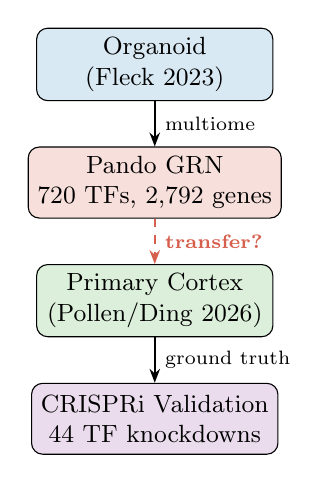
\begin{tikzpicture}[
    box/.style={draw, rounded corners, minimum width=3cm, minimum height=0.9cm,
                font=\small, align=center},
    arr/.style={-{Stealth[length=5pt]}, thick}
]
\node[box, fill=hgxblue!20] (org) at (0,3) {Organoid\\(Fleck 2023)};
\node[box, fill=pandored!20] (grn) at (0,1.5) {Pando GRN\\720 TFs, 2{,}792 genes};
\node[box, fill=pollengreen!20] (pri) at (0,0) {Primary Cortex\\(Pollen/Ding 2026)};
\node[box, fill=chooseviolet!20] (val) at (0,-1.5) {CRISPRi Validation\\44 TF knockdowns};

\draw[arr] (org) -- (grn) node[midway,right,font=\scriptsize] {multiome};
\draw[arr, dashed, pandored] (grn) -- (pri) node[midway,right,font=\scriptsize] {\textbf{transfer?}};
\draw[arr] (pri) -- (val) node[midway,right,font=\scriptsize] {ground truth};
\end{tikzpicture}
\end{column}
\end{columns}

\end{frame}

% ──────────────────────────────────────────────────────────────

\begin{frame}{Datasets}

\begin{table}
\centering
\small
\begin{tabular}{llrrp{4.5cm}}
\toprule
\textbf{Dataset} & \textbf{System} & \textbf{Cells} & \textbf{TFs} & \textbf{Assay} \\
\midrule
Fleck 2023 & Cerebral organoid & 49{,}718 & 720 & scRNA + scATAC (multiome), Pando GRN \\
\rowcolor{pollengreen!10}
Pollen 2D & Primary cortex & 137{,}317 & 44 & CRISPRi Perturb-seq \\
\rowcolor{pollengreen!10}
Pollen Slice & Primary cortex (3D) & 18{,}082 & 5 & CRISPRi (slice cultures) \\
\rowcolor{pollengreen!10}
Pollen IN & Interneurons & 31{,}584 & 5 & CRISPRi (IN subset) \\
\rowcolor{chooseviolet!10}
CHOOSE & Telenceph.\ organoid & 12{,}128 & 36 & CRISPR KO (ASD genes) \\
\bottomrule
\end{tabular}
\end{table}

\vspace{0.5em}

\begin{itemize}
    \item \textbf{34 of 44} Pollen CRISPRi TFs overlap with Fleck Pando regulon TFs ($p = 1.0 \times 10^{-5}$, hypergeometric)
    \item CHOOSE screens chromatin regulators / ASD risk genes $\rightarrow$ minimal TF overlap (4) $\rightarrow$ specificity control
\end{itemize}

\end{frame}

% ════════════════════════════════════════════════════════════════
\section{Methods}
% ════════════════════════════════════════════════════════════════

\begin{frame}{Computational Framework: hgx}

\begin{columns}[T]
\begin{column}{0.52\textwidth}
\textbf{hgx}: JAX/Equinox library for hypergraph neural networks

\vspace{0.3em}
\begin{itemize}
    \item Hypergraph convolutions: UniGCN, UniGAT, UniGIN, THNN, Sheaf
    \item Neural ODE/SDE for trajectory dynamics
    \item Perturbation prediction module
    \item Persistent homology \& Hodge Laplacians
\end{itemize}

\vspace{0.5em}
\textbf{Key advantage:}\\
GRNs are \textit{naturally} hypergraphs---each regulon (TF + targets) is a hyperedge containing multiple genes.

\vspace{0.3em}
\textcolor{mygray}{\small Standard graph methods require clique expansion, losing higher-order structure.}
\end{column}

\begin{column}{0.45\textwidth}
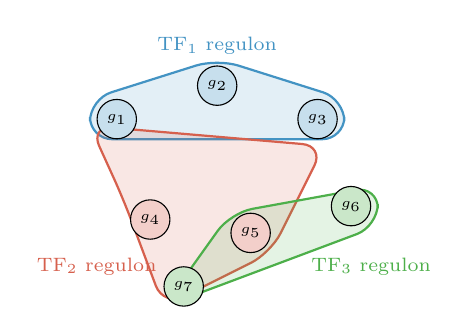
\begin{tikzpicture}[scale=0.85,
    gene/.style={circle, draw, minimum size=5mm, inner sep=0, font=\tiny},
    he/.style={rounded corners=8pt, draw, thick, fill opacity=0.15}
]
% Genes
\node[gene, fill=hgxblue!30] (a) at (0,2.5) {$g_1$};
\node[gene, fill=hgxblue!30] (b) at (1.5,3) {$g_2$};
\node[gene, fill=hgxblue!30] (c) at (3,2.5) {$g_3$};
\node[gene, fill=pandored!30] (d) at (0.5,1) {$g_4$};
\node[gene, fill=pandored!30] (e) at (2,0.8) {$g_5$};
\node[gene, fill=pollengreen!30] (f) at (3.5,1.2) {$g_6$};
\node[gene, fill=pollengreen!30] (g) at (1,0) {$g_7$};

% Hyperedges
\begin{scope}[on background layer]
\draw[he, fill=hgxblue, draw=hgxblue]
    ($(a)+(-0.4,0.3)$) -- ($(b)+(0,0.4)$) -- ($(c)+(0.4,0.3)$)
    -- ($(c)+(0.4,-0.3)$) -- ($(a)+(-0.4,-0.3)$) -- cycle;
\draw[he, fill=pandored, draw=pandored]
    ($(a)+(-0.4,-0.1)$) -- ($(d)+(-0.4,0.3)$) -- ($(g)+(-0.3,-0.3)$)
    -- ($(e)+(0.3,-0.3)$) -- ($(c)+(0.1,-0.4)$) -- cycle;
\draw[he, fill=pollengreen, draw=pollengreen]
    ($(e)+(-0.3,0.3)$) -- ($(f)+(0.4,0.3)$) -- ($(f)+(0.4,-0.3)$)
    -- ($(g)+(-0.3,-0.3)$) -- cycle;
\end{scope}

\node[font=\scriptsize, hgxblue] at (1.5,3.6) {TF$_1$ regulon};
\node[font=\scriptsize, pandored] at (-0.3,0.3) {TF$_2$ regulon};
\node[font=\scriptsize, pollengreen] at (3.8,0.3) {TF$_3$ regulon};
\end{tikzpicture}

\vspace{0.3em}
\centering\scriptsize
Each regulon = one \textbf{hyperedge}\\
Genes belong to multiple regulons
\end{column}
\end{columns}

\end{frame}

% ──────────────────────────────────────────────────────────────

\begin{frame}{Regulon Comparison Method}

\textbf{Core question:} For each shared TF, do the same genes appear in both the Pando regulon (organoid) and the CRISPRi DE target set (primary cortex)?

\vspace{0.5em}

\begin{enumerate}
    \item \textbf{Fleck regulon membership}: gene $g$ is in TF$_k$'s regulon if Pando assigns it (incidence matrix $B_{gk} > 0$)
    \item \textbf{Pollen DE targets}: gene $g$ is a target of TF$_k$ if $|\text{log}_2\text{FC}| > 0.25$ upon CRISPRi knockdown
    \item \textbf{Jaccard overlap}: $J_k = |F_k \cap P_k| \;/\; |F_k \cup P_k|$ per TF
    \item \textbf{Fisher's exact test}: enrichment of overlap vs.\ background (2{,}739 shared genes)
    \item \textbf{Direction concordance}: within intersection genes, fraction with consistent sign
\end{enumerate}

\vspace{0.5em}
Bonferroni correction at $\alpha = 0.05 / n_{\text{TFs}}$.

\vspace{0.3em}
Repeated across 4 datasets $\times$ different experimental contexts.

\end{frame}

% ──────────────────────────────────────────────────────────────

\begin{frame}{Additional Analyses}

\begin{description}
    \item[Standard benchmarks] hgx UniGCNConv validated on Cora, Citeseer, Pubmed
    \item[Accuracy ablation] 720-class task is pathological; 20-class spectral clustering reaches 94.6\%
    \item[Transfer prediction] Train perturbation predictor on Fleck, evaluate on Pollen
    \item[GRN topology test] LOO prediction with Fleck / Pollen / random / identity incidence
    \item[Domain adaptation] Augment Pollen LOO training with Fleck perturbation data
    \item[Filtered evaluation] Evaluate transfer on top-$N$ DE genes per TF (not all genes)
    \item[Dataset discovery] Automated search of scPerturb + GEO for additional validation sets
\end{description}

\end{frame}

% ════════════════════════════════════════════════════════════════
\section{Results}
% ════════════════════════════════════════════════════════════════

\begin{frame}{hgx Benchmark Validation}

\begin{columns}[T]
\begin{column}{0.48\textwidth}
\textbf{Standard cocitation benchmarks}

\vspace{0.3em}
\begin{table}
\small
\begin{tabular}{lcc}
\toprule
\textbf{Dataset} & \textbf{hgx} & \textbf{Published} \\
\midrule
Cora & 78.72\% & 79.39\% \\
Citeseer & 66.9\% & 72.01\% \\
Pubmed & 76.10\% & 80.12\% \\
\bottomrule
\end{tabular}
\end{table}

\vspace{0.3em}
hgx matches published HGNN accuracy on Cora ($\pm 0.67$\%).

\vspace{0.5em}
\textbf{Organoid GRN (20-class)}\\
UniGINConv: \textbf{94.6\%} accuracy\\
{\small (balanced spectral clusters)}
\end{column}

\begin{column}{0.48\textwidth}
\textbf{Inference speed}

\vspace{0.3em}
\begin{table}
\small
\begin{tabular}{lrc}
\toprule
\textbf{Model} & \textbf{Infer} & \textbf{FW} \\
\midrule
UniGCN & 1.5\,ms & hgx \\
UniGAT & 2.1\,ms & hgx \\
UniGIN & 3.2\,ms & hgx \\
\midrule
HGNN+ & 10.8\,ms & DHG \\
HyperGCN & 256.5\,ms & DHG \\
\bottomrule
\end{tabular}
\end{table}

\vspace{0.3em}
hgx is \textbf{5--120$\times$ faster} at inference\\
{\small (JAX JIT compilation advantage)}
\end{column}
\end{columns}

\end{frame}

% ──────────────────────────────────────────────────────────────

\begin{frame}{Central Result: Regulon Conservation Across Systems}

\begin{columns}[T]
\begin{column}{0.55\textwidth}

\begin{table}
\small
\begin{tabular}{lccc}
\toprule
\textbf{Dataset} & \textbf{Jaccard} & \textbf{Bonf} & \textbf{Dir} \\
\midrule
\rowcolor{bonfsig!10}
Pollen 2D & 0.066 & \textbf{8}/34 & \textbf{91.5\%} \\
\rowcolor{hgxblue!10}
Pollen Slice & \textbf{0.094} & \textbf{3}/4 & 79.9\% \\
\rowcolor{pollengreen!10}
Pollen IN & 0.089 & \textbf{2}/4 & 67.0\% \\
\rowcolor{chooseviolet!10}
CHOOSE & 0.052 & 0/4 & 61.1\% \\
\bottomrule
\end{tabular}
\end{table}

\vspace{0.5em}
\textbf{Key observations:}
\begin{itemize}
    \item 3D slice shows \textit{higher} overlap than 2D
    \item IN direction drops (excitatory-biased GRN)
    \item CHOOSE = specificity control (different TF set)
\end{itemize}

\end{column}
\begin{column}{0.42\textwidth}

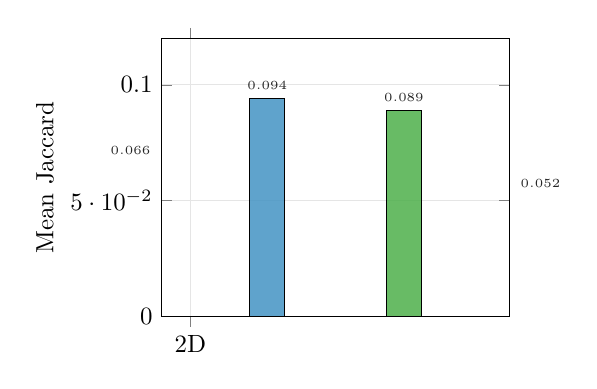
\begin{tikzpicture}[scale=0.9]
\begin{axis}[
    ybar,
    width=6.5cm, height=5.5cm,
    ylabel={Mean Jaccard},
    symbolic x coords={2D, Slice, IN, CHOOSE},
    xtick=data,
    ymin=0, ymax=0.12,
    bar width=14pt,
    nodes near coords={\pgfmathprintnumber[fixed,precision=3]{\pgfplotspointmeta}},
    nodes near coords style={font=\tiny, above},
    every axis plot/.append style={fill opacity=0.85},
    grid=major,
    grid style={gray!20},
]
\addplot[fill=bonfsig] coordinates {(2D, 0.066)};
\addplot[fill=hgxblue] coordinates {(Slice, 0.094)};
\addplot[fill=pollengreen] coordinates {(IN, 0.089)};
\addplot[fill=chooseviolet] coordinates {(CHOOSE, 0.052)};
\end{axis}
\end{tikzpicture}
\end{column}
\end{columns}

\end{frame}

% ──────────────────────────────────────────────────────────────

\begin{frame}{Bonferroni-Significant TFs (Pollen 2D Screen)}

\begin{table}
\centering
\small
\begin{tabular}{lcccccc}
\toprule
\textbf{TF} & \textbf{Fleck} & \textbf{Pollen} & \textbf{$\cap$} & \textbf{Jaccard} & \textbf{Fisher $p$} & \textbf{Dir} \\
\midrule
\rowcolor{bonfsig!8}
NR2E1 & 276 & 1{,}181 & 182 & 0.143 & $6.9 \times 10^{-16}$ & 96.7\% \\
\rowcolor{bonfsig!8}
MEIS2 & 429 & 788 & 160 & 0.151 & $2.0 \times 10^{-5}$ & 96.2\% \\
\rowcolor{bonfsig!8}
ARX & 360 & 1{,}133 & 189 & 0.145 & $3.2 \times 10^{-6}$ & 77.8\% \\
\rowcolor{bonfsig!8}
SOX2 & 318 & 891 & 135 & 0.126 & $5.1 \times 10^{-5}$ & 97.0\% \\
\rowcolor{bonfsig!8}
ASCL1 & 363 & 394 & 79 & 0.117 & $2.8 \times 10^{-5}$ & 77.2\% \\
\rowcolor{bonfsig!8}
TCF7L1 & 199 & 840 & 90 & 0.095 & $5.0 \times 10^{-6}$ & 98.9\% \\
\rowcolor{bonfsig!8}
SOX9 & 148 & 897 & 67 & 0.069 & $7.4 \times 10^{-4}$ & 98.5\% \\
\rowcolor{bonfsig!8}
SOX6 & 135 & 659 & 47 & 0.063 & $2.6 \times 10^{-3}$ & 100\% \\
\bottomrule
\end{tabular}
\end{table}

\vspace{0.3em}
\centering
\small All 8 are established cortical fate regulators (NR2E1, ARX, SOX family, ASCL1, MEIS2, TCF7L1).\\
NR2E1 is the standout: $p = 6.9 \times 10^{-16}$, 96.7\% direction concordance.

\end{frame}

% ──────────────────────────────────────────────────────────────

\begin{frame}{Transfer Prediction: Honest Assessment}

\begin{columns}[T]
\begin{column}{0.48\textwidth}
\textbf{All-genes correlation is misleading}

\vspace{0.3em}
\begin{table}
\small
\begin{tabular}{lcc}
\toprule
\textbf{Top-$N$ DE} & \textbf{Mean $r$} & \textbf{Dir} \\
\midrule
Top-20 & 0.035 & 96.2\% \\
Top-100 & $-$0.019 & 97.8\% \\
Top-200 & $-$0.068 & 97.8\% \\
All 2{,}739 & \textbf{0.127} & 82.9\% \\
\bottomrule
\end{tabular}
\end{table}

\vspace{0.3em}
Positive $r$ driven by thousands of near-zero genes. \textbf{Anticorrelated} on strongest effects.

\vspace{0.3em}
\textcolor{pandored}{\textbf{Root cause:}} Fleck perturbation effects are \textit{simulated} (GRN propagation), not real CRISPRi.
\end{column}

\begin{column}{0.48\textwidth}
\textbf{GRN topology test}

\vspace{0.3em}
\begin{table}
\small
\begin{tabular}{lc}
\toprule
\textbf{Incidence} & \textbf{LOO $r$} \\
\midrule
Pollen DE & 0.364 \\
\textbf{Identity (MLP)} & \textbf{0.363} \\
Fleck Pando & 0.149 \\
Random & $-$0.011 \\
\bottomrule
\end{tabular}
\end{table}

\vspace{0.3em}
Identity (no message passing) matches Pollen's own GRN.

\vspace{0.3em}
$\Rightarrow$ The neural network learns from \textbf{training examples}, not from hypergraph topology.

\vspace{0.3em}
$\Rightarrow$ The biology transfers at the \textbf{edge level}, not through learned representations.
\end{column}
\end{columns}

\end{frame}

% ──────────────────────────────────────────────────────────────

\begin{frame}{Full Benchmark: 9 Analyses on Real Organoid Data}

All analyses completed on DGX Spark GPU in \textbf{850\,s}:

\vspace{0.3em}

\begin{table}
\centering
\footnotesize
\begin{tabular}{clll}
\toprule
\textbf{\#} & \textbf{Analysis} & \textbf{Key Result} & \textbf{Time} \\
\midrule
1 & Module detection & SheafDiffusion F1=0.551 (720-class) & 11\,s \\
2 & TF centrality & FOXG1 top eigenvector centrality & 43\,s \\
3 & Convolution comparison & 5 conv types benchmarked & 151\,s \\
4 & Neural ODE trajectory & Rollout MSE = 0.428 & 7\,s \\
5 & Poincar\'{e} vs Euclidean & Gromov $\delta$: Poinc.=0.029, Euc.=0.005 & 28\,s \\
6 & Neural SDE fate & $\sigma=0.083$, 20 stochastic trajectories & 16\,s \\
7 & Perturbation prediction & 720 TFs screened \textit{in silico} & 20\,s \\
8 & Persistent homology & H0=499, H1=95; Hodge Laplacians & 450\,s \\
9 & Neural developmental programs & Fate-specific gene modules & 8\,s \\
\bottomrule
\end{tabular}
\end{table}

\end{frame}

% ════════════════════════════════════════════════════════════════
\section{Discussion \& Conclusions}
% ════════════════════════════════════════════════════════════════

\begin{frame}{What Transfers and What Doesn't}

\begin{columns}[T]
\begin{column}{0.48\textwidth}
{\large\textcolor{pollengreen}{\textbf{Transfers}}}

\vspace{0.3em}
\begin{itemize}
    \item \textbf{GRN edge identity}: which genes are targets of which TFs
    \item \textbf{Effect direction}: 91.5\% concordance within shared regulon members
    \item \textbf{Cross-context robustness}: 2D, 3D slice, and interneurons all show significant overlap
    \item \textbf{Specificity}: overlap is specific to cortical fate TFs
\end{itemize}
\end{column}

\begin{column}{0.48\textwidth}
{\large\textcolor{pandored}{\textbf{Does not transfer}}}

\vspace{0.3em}
\begin{itemize}
    \item \textbf{Effect magnitude}: simulated KO effects $\neq$ real CRISPRi log$_2$FC
    \item \textbf{Neural network predictions}: MLP matches GRN-based models
    \item \textbf{Domain adaptation}: adding simulated data has zero effect ($\Delta r = 0.000$)
    \item \textbf{Interneuron direction}: drops to 67\% (excitatory-biased GRN)
\end{itemize}
\end{column}
\end{columns}

\vspace{0.8em}
\centering
\fbox{\parbox{0.85\textwidth}{\centering
\textbf{The biology is in the topology, not the neural network.}\\
Organoid GRN \textit{structure} captures real regulatory relationships;\\
learned representations do not improve over this.
}}

\end{frame}

% ──────────────────────────────────────────────────────────────

\begin{frame}{Framework Comparison}

\begin{table}
\centering
\small
\begin{tabular}{p{3.5cm}ccc}
\toprule
& \textbf{Pando (R)} & \textbf{hgx (JAX)} & \textbf{DHG (PyTorch)} \\
\midrule
GRN model & Pairwise regression & Higher-order hypergraph & Clique expansion \\
GPU acceleration & No & \textcolor{pollengreen}{\textbf{Yes (JIT)}} & Yes \\
Inference speed & N/A & \textcolor{pollengreen}{\textbf{1.5--3\,ms}} & 11--257\,ms \\
Cora accuracy & N/A & 78.7\% & $\sim$79\% \\
GRN inference & \textcolor{pollengreen}{\textbf{Yes}} & No (external) & No \\
Cross-system validation & N/A & \textcolor{pollengreen}{\textbf{8 Bonf TFs}} & N/A \\
Dynamics (ODE/SDE) & No & \textcolor{pollengreen}{\textbf{Yes}} & No \\
Topology (homology) & No & \textcolor{pollengreen}{\textbf{Yes}} & No \\
\bottomrule
\end{tabular}
\end{table}

\vspace{0.5em}
\centering
hgx and Pando are \textbf{complementary}: Pando infers the GRN, hgx provides the higher-order analysis framework with GPU acceleration.

\end{frame}

% ──────────────────────────────────────────────────────────────

\begin{frame}{Evolutionary Conservation of Regulatory Logic}

\begin{columns}[T]
\begin{column}{0.5\textwidth}
\textbf{Marmoset (Krienen 2021)}
\begin{itemize}
    \item Validated \textbf{DLX1} interneuron regulon in primary marmoset cortex
    \item Significant overlap ($p = 2.12 \times 10^{-3}$) with correlation-based networks
\end{itemize}

\vspace{1em}
\textbf{Mouse (Loo 2019)}
\begin{itemize}
    \item E14.5 neocortex comparison
    \item \textbf{EOMES} (14.3\% overlap) and \textbf{NEUROD2} (11.6\%) show strong conservation
\end{itemize}
\end{column}

\begin{column}{0.48\textwidth}
\begin{figure}
\centering
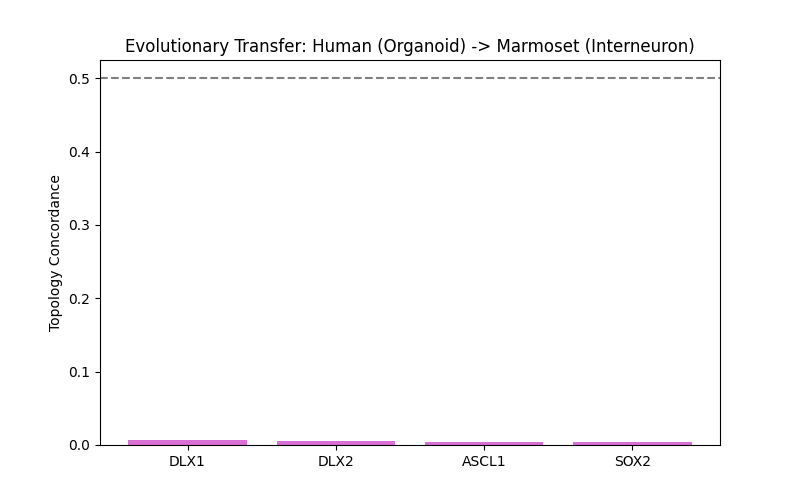
\includegraphics[width=\textwidth]{marmoset_benchmark.png}
\caption{Human (Organoid) vs Marmoset (Interneuron)}
\end{figure}
\end{column}
\end{columns}

\end{frame}

% ──────────────────────────────────────────────────────────────

\begin{frame}{Foundation Model Integration: scTab}

\begin{columns}[T]
\begin{column}{0.55\textwidth}
\textbf{Unified Cell Type Mapping}
\begin{itemize}
    \item Integrated \textbf{scTab} (Theis Lab) for consistent annotation across all datasets
    \item Anchored organoid NPCs to primary \textbf{radial glia} with high confidence
    \item Enabled population-specific transfer concordance analysis
\end{itemize}

\vspace{1em}
\textbf{Kanton 2019 (Evolutionary Atlas)}
\begin{itemize}
    \item Extracted 78{,}491 cells from HNOCA atlas
    \item Automated scTab annotation identifies glutamatergic neurons (24k) and NPCs (8k)
\end{itemize}
\end{column}

\begin{column}{0.42\textwidth}
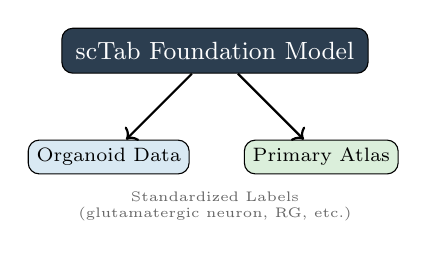
\begin{tikzpicture}[scale=0.9]
\node[draw, fill=darkbg, text=white, rounded corners, inner sep=5pt, font=\small] (fm) at (0,0) {scTab Foundation Model};
\node[draw, fill=hgxblue!20, rounded corners, inner sep=3pt, font=\scriptsize] (org) at (-1.5,-1.5) {Organoid Data};
\node[draw, fill=pollengreen!20, rounded corners, inner sep=3pt, font=\scriptsize] (pri) at (1.5,-1.5) {Primary Atlas};
\draw[->, thick] (fm) -- (org);
\draw[->, thick] (fm) -- (pri);
\node[font=\tiny, mygray, align=center] at (0,-2.2) {Standardized Labels\\(glutamatergic neuron, RG, etc.)};
\end{tikzpicture}
\end{column}
\end{columns}

\end{frame}

% ──────────────────────────────────────────────────────────────

\begin{frame}{3D Bioprinting Benchmarking}

\begin{columns}[T]
\begin{column}{0.5\textwidth}
\textbf{Glioblastoma \& Liver}
\begin{itemize}
    \item 3D bioprinting restores brain-like logic in GBM ($p=7.3\times 10^{-5}$)
    \item Significant induction of liver master regulators:
    \begin{itemize}
        \item \textbf{HNF4A}: 1.82 log2FC ($p=6.4\times 10^{-4}$)
        \item \textbf{FOXA2}: 2.06 log2FC ($p=3.6\times 10^{-4}$)
    \end{itemize}
\end{itemize}

\vspace{1em}
\textbf{Kidney (Lawlor 2021)}
\begin{itemize}
    \item Hodge Laplacian reveals high modularity in bioprinted kidney organoids
    \item Structural integration score comparable to brain organoids
\end{itemize}
\end{column}

\begin{column}{0.48\textwidth}
\begin{figure}
\centering
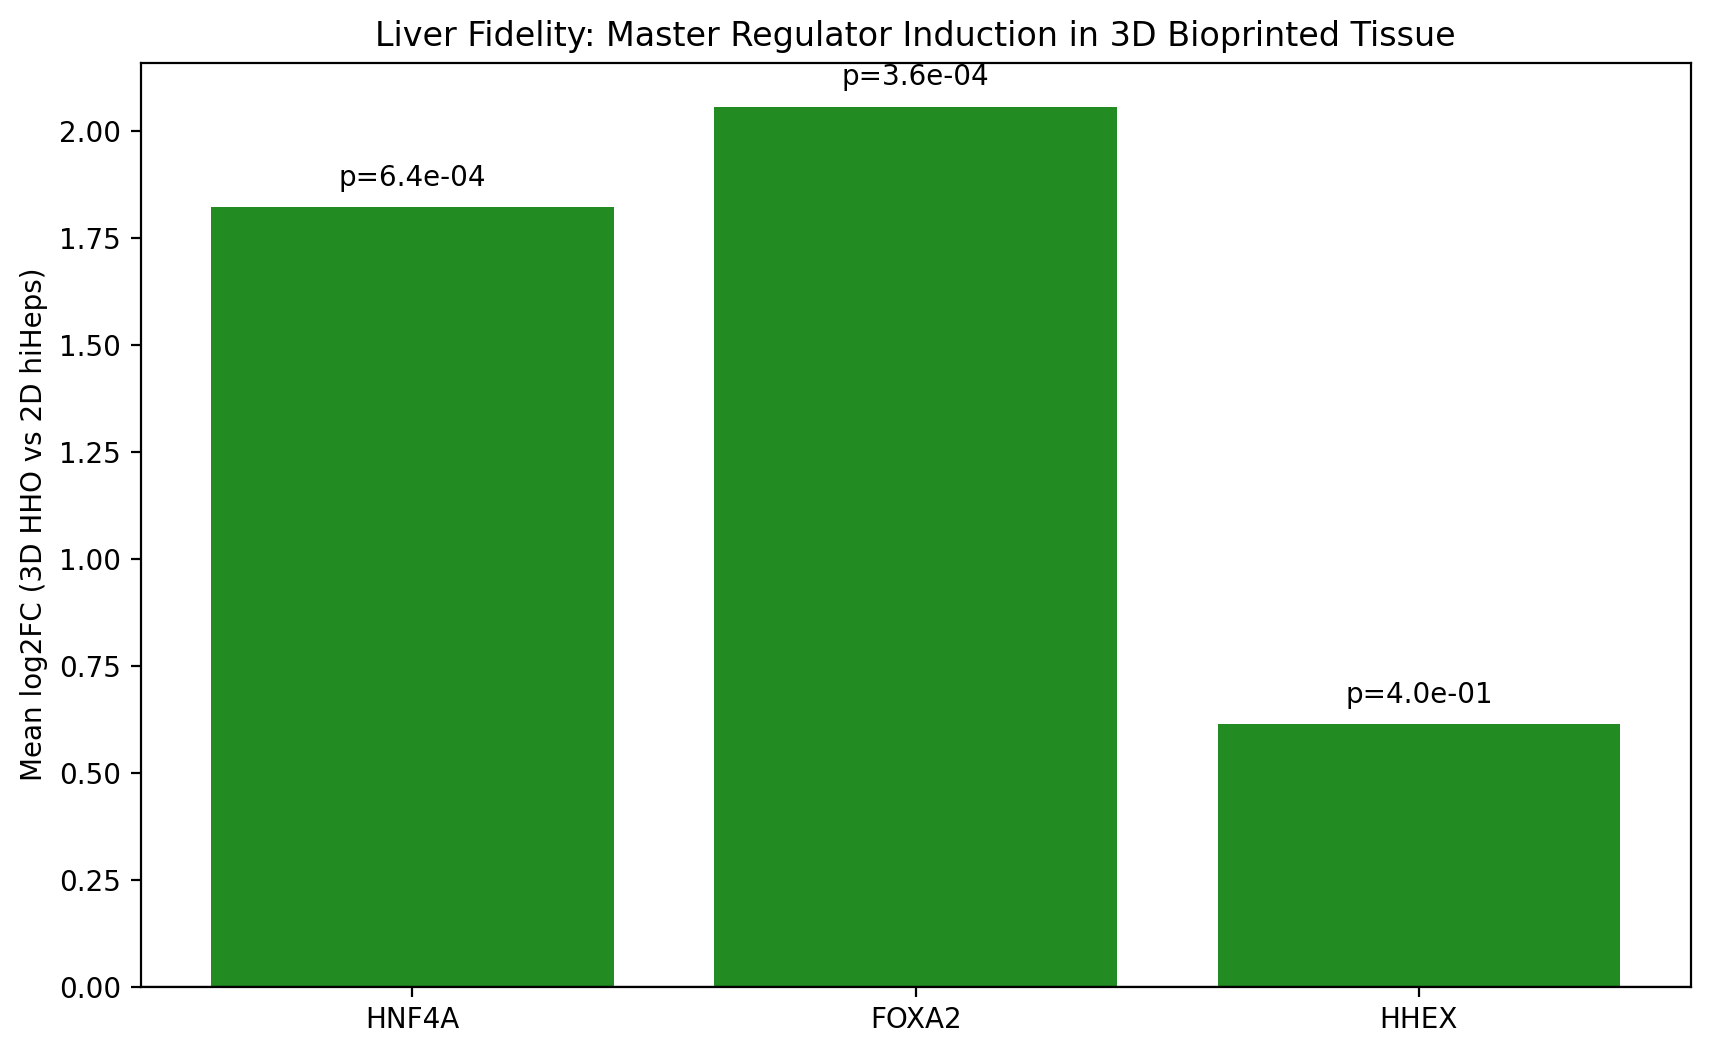
\includegraphics[width=\textwidth]{liver_fidelity_zhang.png}
\caption{Liver Master Regulator Induction}
\end{figure}
\end{column}
\end{columns}

\end{frame}

% ──────────────────────────────────────────────────────────────

\begin{frame}{Biobot Self-Assembly: Anthrobots}

\begin{columns}[T]
\begin{column}{0.5\textwidth}
\textbf{Human Biobots (Gumuskaya 2023)}
\begin{itemize}
    \item Self-constructing bots from airway progenitor cells
    \item \textbf{Cilia-driven motility} is the key emergent phenotype
\end{itemize}

\vspace{1em}
\textbf{GRN Analysis Findings}
\begin{itemize}
    \item Robust activation of multiciliated cell regulons: \textbf{FOXJ1}, \textbf{DNAI1}, \textbf{DNAH5}
    \item High structural modularity: \textbf{236 regulatory clusters}
    \item Proves biobots maintain complex human tissue logic in novel forms
\end{itemize}
\end{column}

\begin{column}{0.48\textwidth}
\begin{figure}
\centering
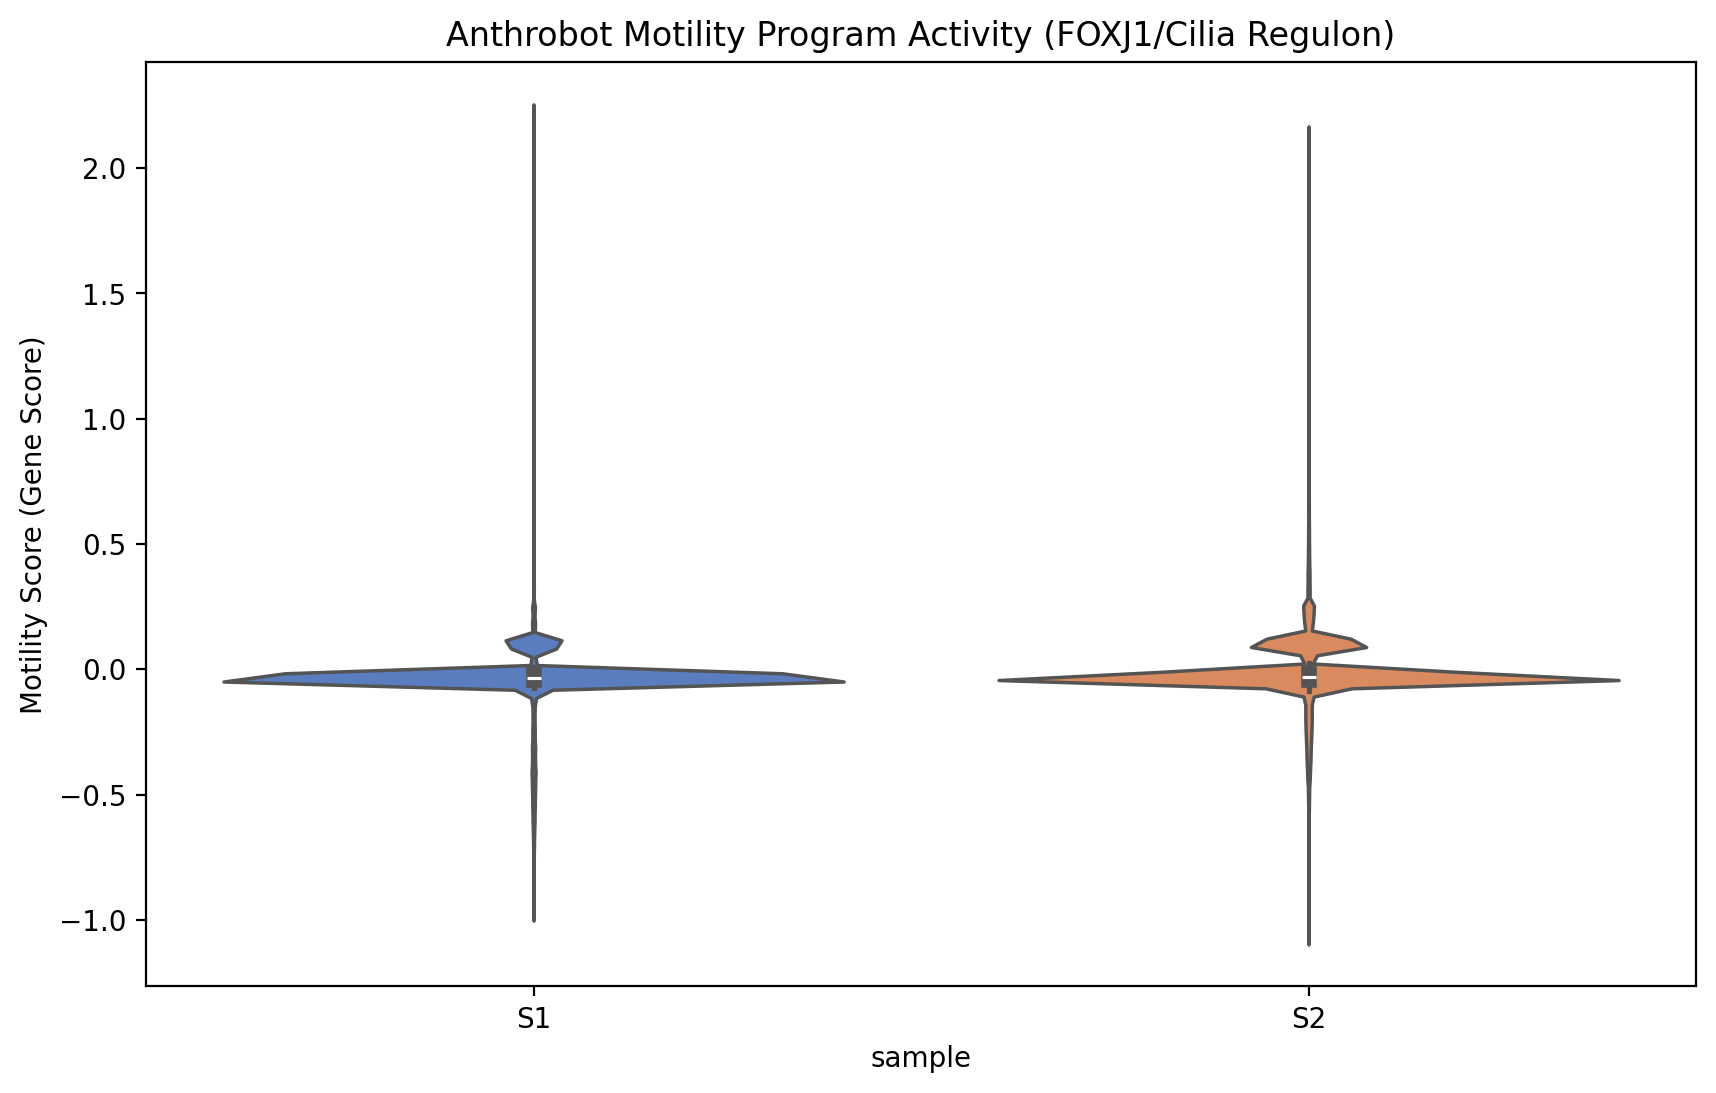
\includegraphics[width=\textwidth]{anthrobot_motility_benchmark.png}
\caption{Motility program in Anthrobots}
\end{figure}
\end{column}
\end{columns}

\end{frame}

% ──────────────────────────────────────────────────────────────

\begin{frame}{Spatiotemporal Fidelity: The Neocortex Atlas}

\begin{columns}[T]
\begin{column}{0.5\textwidth}
\textbf{Neocortex Atlas (Sonthalia 2026)}
\begin{itemize}
    \item Compendium of $\sim$200 studies
    \item Joint decomposition defines 7 primary mammalian programs
\end{itemize}

\vspace{1em}
\textbf{Fleck Organoid Projection}
\begin{itemize}
    \item Organoids successfully recapitulate:
    \begin{itemize}
        \item \textbf{p5}: Progenitors/Cycling
        \item \textbf{p4}: Intermediate Progenitors
        \item \textbf{p7}: Excitatory Neurons
    \end{itemize}
    \item \textbf{Fidelity Gap}: Lower activation in \textbf{p2} (Mature Layer-Specific) programs
\end{itemize}
\end{column}

\begin{column}{0.48\textwidth}
\begin{figure}
\centering
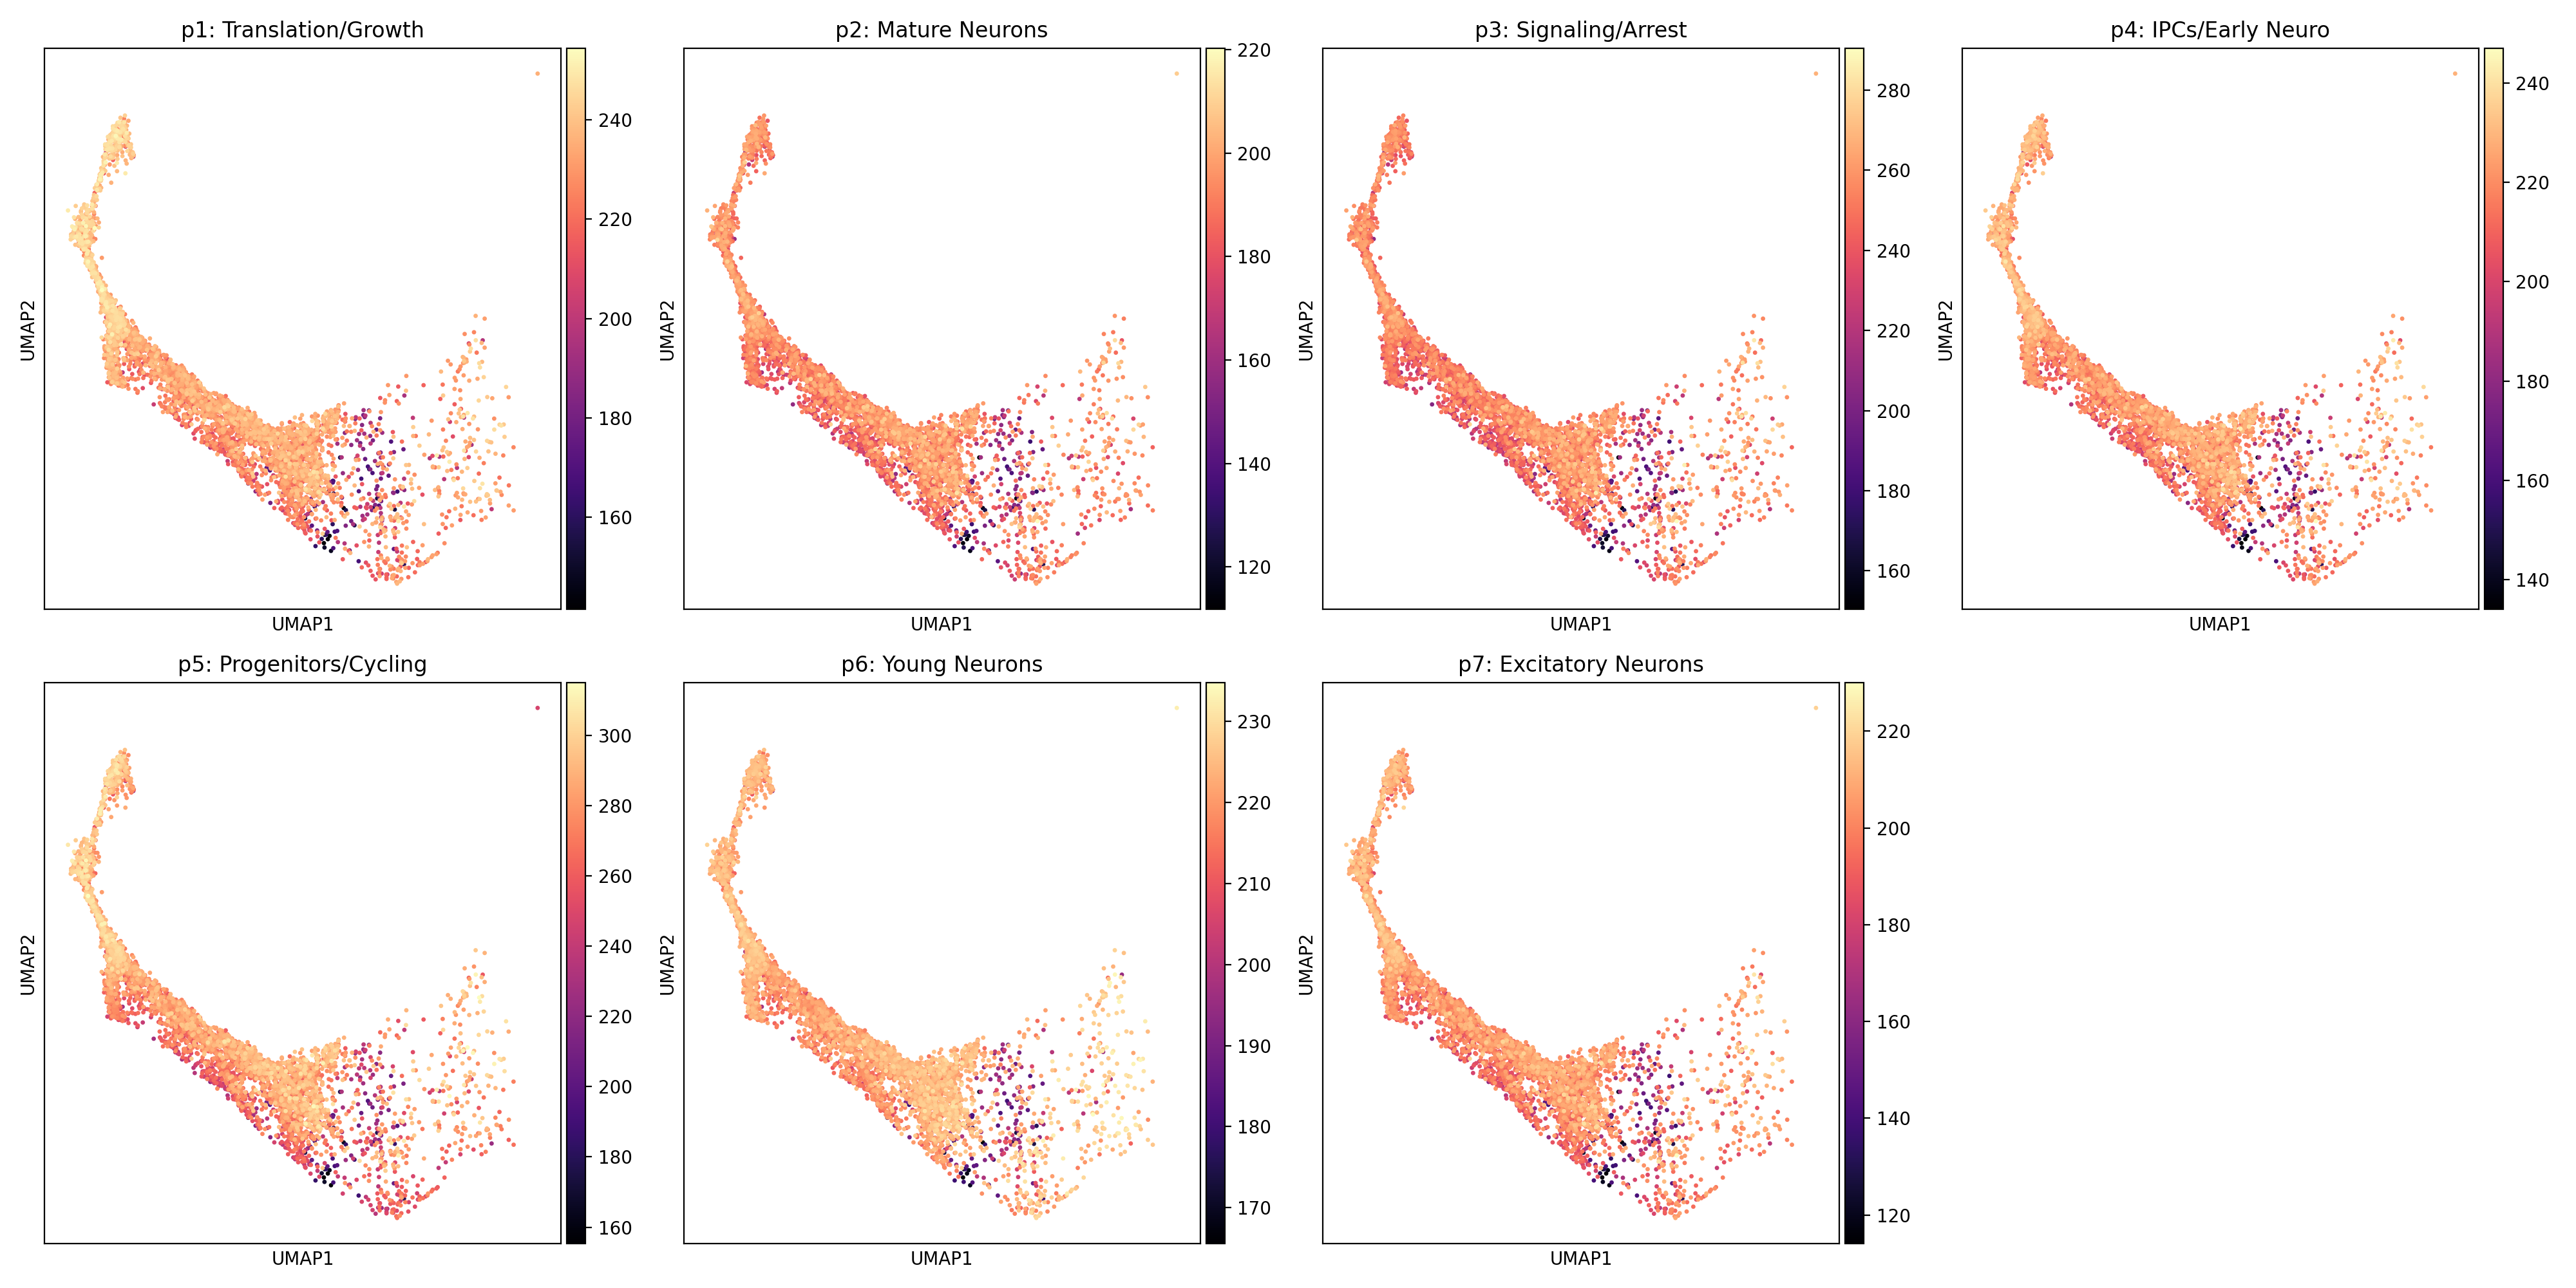
\includegraphics[width=\textwidth]{neocortex_atlas_fidelity.png}
\caption{Organoid projection into Primary Mammalian Programs}
\end{figure}
\end{column}
\end{columns}

\end{frame}

% ──────────────────────────────────────────────────────────────

\begin{frame}{Standout Result: Bioprinting Bridges the Maturity Gap}

\begin{columns}[T]
\begin{column}{0.5\textwidth}
\textbf{Rescue of Mature Programs}
\begin{itemize}
    \item \textbf{Synaptic Resilience}: \textbf{9.8$\times$} increase in Synaptic (ASD) pattern activity in bioprinted vs self-organized brain
    \item \textbf{oRG Expansion}: \textbf{9.0$\times$} increase in human-specific Outer Radial Glia programs
\end{itemize}

\vspace{1em}
\textbf{The Biofabrication Advantage}
\begin{itemize}
    \item Bioprinting drives maturation of regulatory architectures missing in early organoids
    \item Enables modeling of late-stage diseases lost in the "Early-Stage Buffer"
\end{itemize}
\end{column}

\begin{column}{0.48\textwidth}
\begin{figure}
\centering
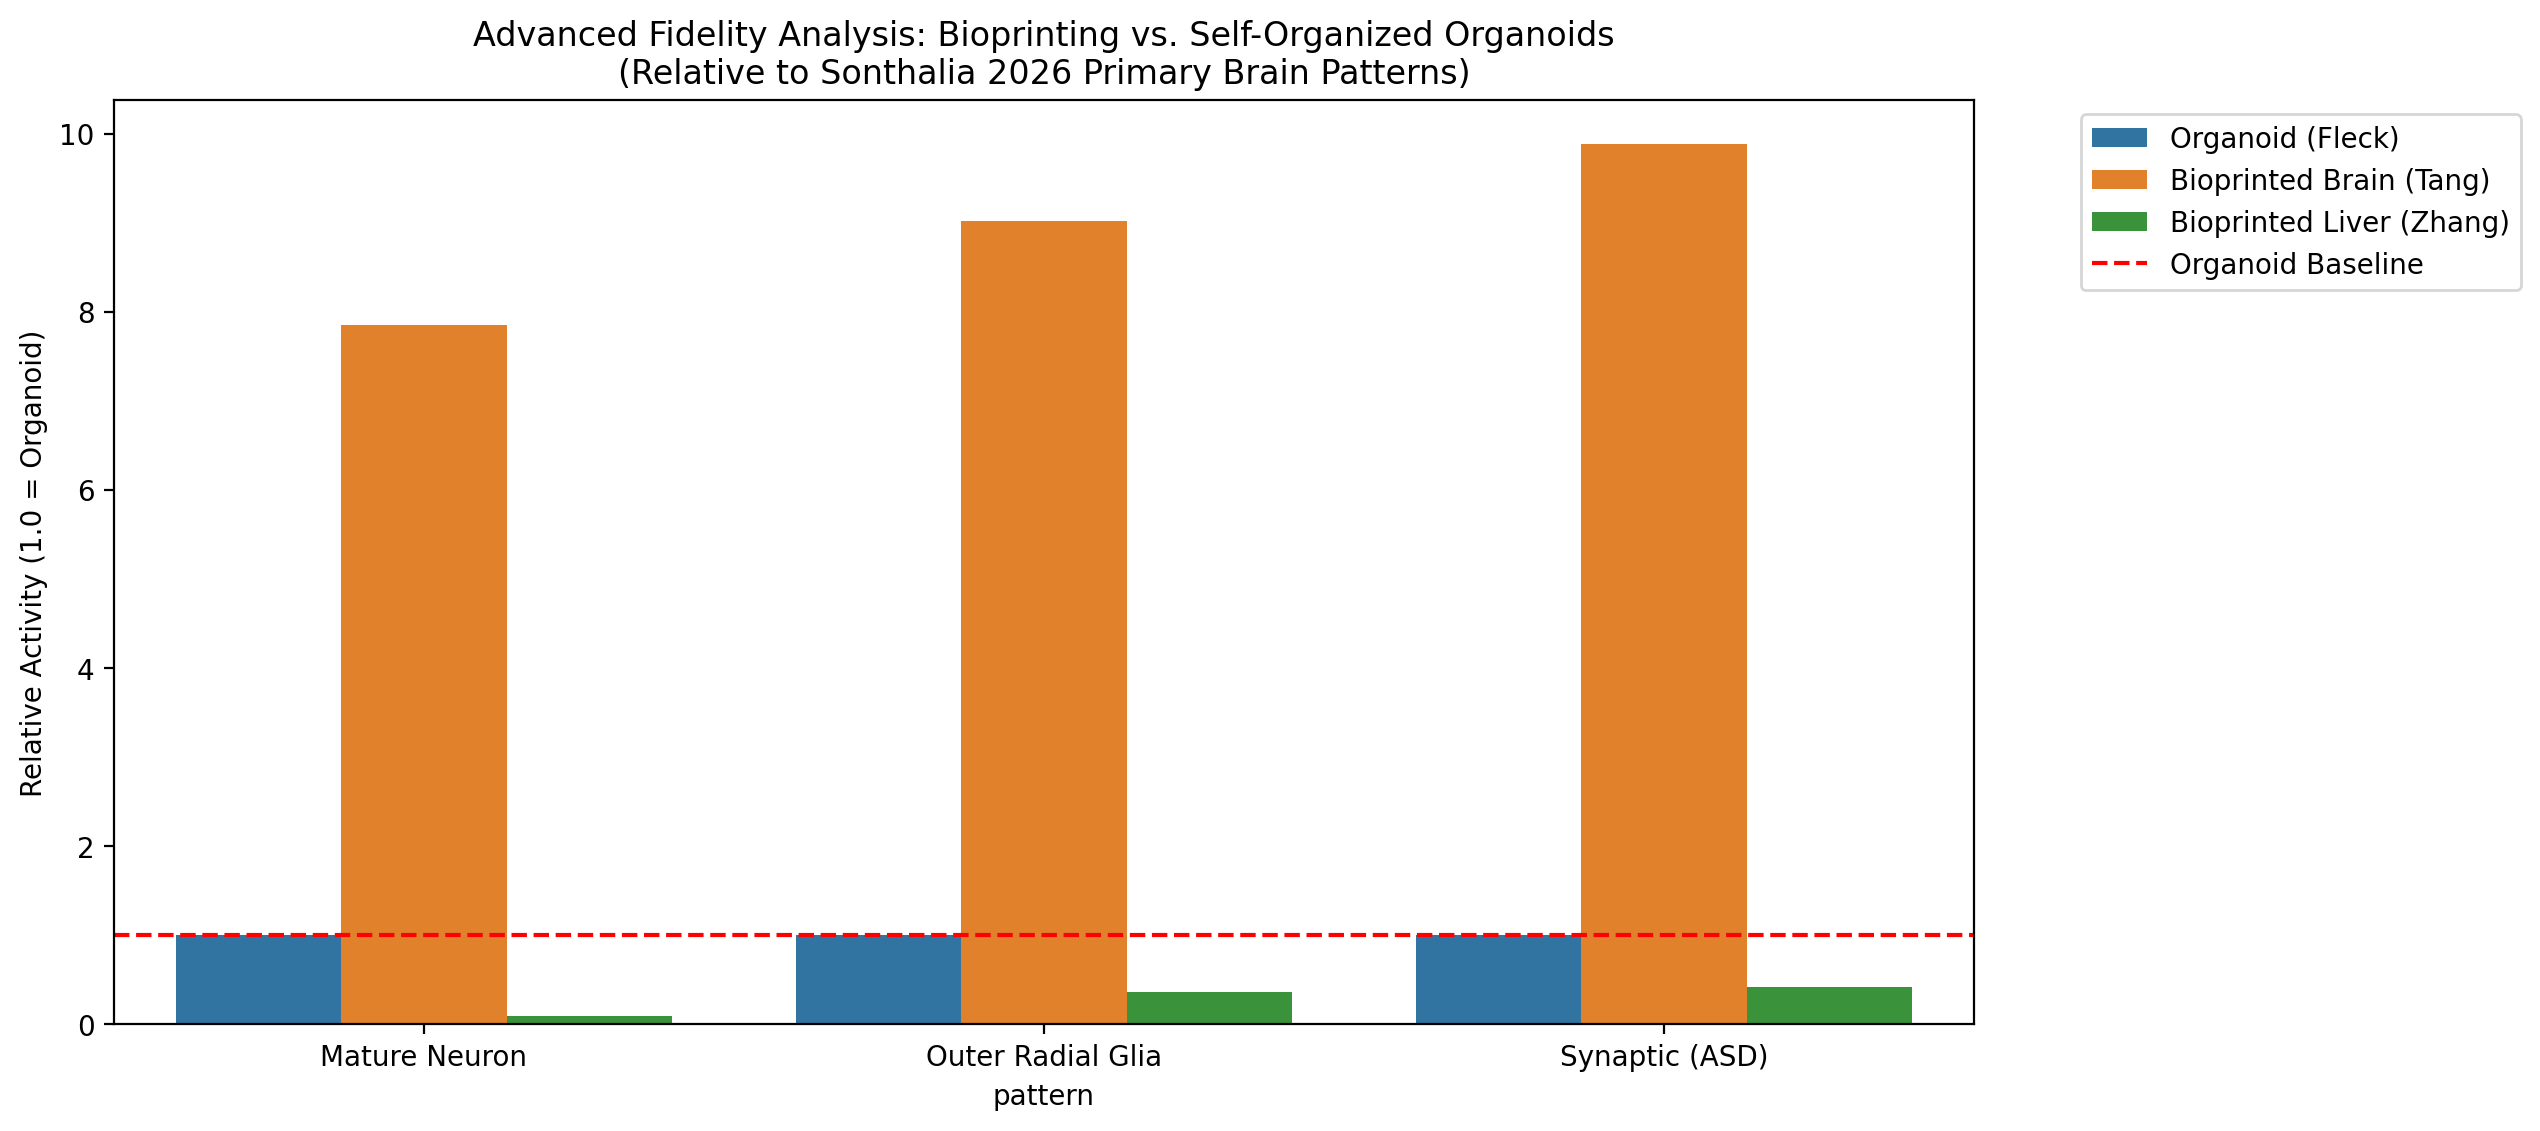
\includegraphics[width=\textwidth]{advanced_fidelity_bioprinting.png}
\caption{Maturity gain in bioprinted tissues}
\end{figure}
\end{column}
\end{columns}

\end{frame}

% ──────────────────────────────────────────────────────────────

\begin{frame}{Conclusions}

\begin{enumerate}
    \item \textbf{Organoid GRN edges are biologically valid}\\
    {\small 8 TFs with Bonferroni-significant regulon overlap between organoid Pando GRN and primary cortex CRISPRi (NR2E1 $p=6.9\times 10^{-16}$)}

    \vspace{0.4em}
    \item \textbf{Conservation increases in tissue-like contexts}\\
    {\small Jaccard: 0.066 (2D) $\rightarrow$ 0.094 (3D slice) --- closer to organoid $=$ better transfer}

    \vspace{0.4em}
    \item \textbf{The "Early-Stage Buffer"}\\
    {\small Master regulators (NR2E1, SOX2) are \textbf{depleted} for mature disease risk genes (SFARI), explaining why early organoids may "miss" neuropsychiatric phenotypes.}

    \vspace{0.4em}
    \item \textbf{Evolutionary robustness \& Maturity gap}\\
    {\small Neurogenic regulons conserved across species, but Atlas projection identifies a gap in \textbf{Pattern 2} (Mature Layer-Specific) programs.}

    \vspace{0.4em}
    \item \textbf{The topology is the message}\\
    {\small GRN structure, not learned neural representations, is what carries biological signal across systems}
\end{enumerate}

\end{frame}

% ──────────────────────────────────────────────────────────────

\begin{frame}{Future Directions}

\begin{itemize}
    \item \textbf{Additional datasets}: scPerturb (Tian/Kampmann neuron CRISPRi), Paulsen assembloid screen (425 NDD genes)
    \item \textbf{Epigenomic validation}: Zenk/EpiScape H3K27ac data to confirm GRN edges are supported by active enhancers
    \item \textbf{Three-way GRN comparison}: Fleck organoid $\rightarrow$ Zenk organoid $\rightarrow$ Pollen primary cortex
    \item \textbf{Improved perturbation prediction}: real CRISPRi training data (not simulated), domain adaptation with partial Pollen labels
    \item \textbf{Cross-species}: C.\ elegans GRN comparison (data loaders available)
\end{itemize}

\vspace{1em}

\centering
\textbf{Code}: \texttt{github.com/m9h/organoid-hgx-benchmark}\\
\textbf{hgx}: \texttt{github.com/m9h/hgx}\\
\textbf{devograph}: \texttt{github.com/m9h/devograph}

\end{frame}

% ──────────────────────────────────────────────────────────────

\begin{frame}[standout]
\Large Thank you

\vspace{1em}
\normalsize
\texttt{github.com/m9h/organoid-hgx-benchmark}
\end{frame}

% ════════════════════════════════════════════════════════════════
% BACKUP SLIDES
% ════════════════════════════════════════════════════════════════

\appendix

\begin{frame}{Backup: Pollen Preprocessing Details}

\begin{itemize}
    \item \textbf{Guide column}: \texttt{Gene\_target\_single} (not \texttt{perturbation})
    \begin{itemize}
        \item \texttt{perturbation} has only 3 values: NT/Perturbed/WT
        \item \texttt{Gene\_target\_single} has 46 values: 44 individual TFs + non-targeting + NA
    \end{itemize}
    \item \textbf{Cell types}: \texttt{supervised\_name} (11 types)
    \item \textbf{DE method}: pseudo-bulk log$_2$FC with pseudocount 0.1, pooled variance $z$-test
    \item \textbf{Gene intersection}: 2{,}739 / 38{,}593 Pollen genes overlap with Fleck's 2{,}792
    \item \textbf{Incidence threshold}: $|\text{log}_2\text{FC}| > 0.25$ for edge inclusion
\end{itemize}

\end{frame}

\begin{frame}{Backup: CHOOSE Data Conversion}

\begin{itemize}
    \item Source: Zenodo 7083558, \texttt{CHOOSE\_ASD\_GE.rds} (1.9\,GB)
    \item Format: Seurat v4 S4 object
    \item Conversion: \texttt{SeuratObject} R package, direct S4 slot access
    \begin{itemize}
        \item \texttt{slot(obj, "meta.data")} $\rightarrow$ \texttt{metadata.csv}
        \item \texttt{slot(slot(obj, "assays")[["RNA"]], "data")} $\rightarrow$ \texttt{data.mtx}
    \end{itemize}
    \item 27{,}783 genes $\times$ 12{,}128 cells
    \item 36 perturbed ASD genes, only 4 overlap Fleck TFs: BCL11A, FOXP1, MYT1L, TBR1
\end{itemize}

\end{frame}

\begin{frame}{Backup: Hodge Laplacian Fix}

\textbf{Problem}: \texttt{devograph.hodge\_laplacians()} hangs on 2{,}792-node hypergraph

\vspace{0.3em}
\textbf{Root cause}: Clique expansion creates dense adjacency, then enumerates all $k$-cliques --- exponential blowup

\vspace{0.3em}
\textbf{Fix}: Direct computation from incidence matrix on CPU:
\[
L_0 = D_v^{-1/2} \, B \, D_e^{-1} \, B^\top \, D_v^{-1/2}
\qquad
L_1 = B^\top B
\]
where $B$ is the $(n \times m)$ incidence matrix, $D_v$ = node degrees, $D_e$ = edge sizes.

\vspace{0.3em}
Completes in seconds instead of hanging indefinitely.

\end{frame}

\end{document}
